% interactapasample.tex
% v1.05 - August 2017

\documentclass[]{interact}

\usepackage{multirow}
\usepackage{epstopdf}% To incorporate .eps illustrations using PDFLaTeX, etc.
\usepackage[caption=false]{subfig}% Support for small, `sub' figures and tables
%\usepackage[nolists,tablesfirst]{endfloat}% To `separate' figures and tables from text if required
%\usepackage[doublespacing]{setspace}% To produce a `double spaced' document if required
%\setlength\parindent{24pt}% To increase paragraph indentation when line spacing is doubled

%\usepackage[longnamesfirst,sort]{natbib}% Citation support using natbib.sty
%\bibpunct[, ]{(}{)}{;}{a}{,}{,}% Citation support using natbib.sty
%\renewcommand\bibfont{\fontsize{10}{12}\selectfont}% To set the list of references in 10 point font using natbib.sty

\usepackage[natbibapa,nodoi]{apacite}% Citation support using apacite.sty. Commands using natbib.sty MUST be deactivated first!
\setlength\bibhang{12pt}% To set the indentation in the list of references using apacite.sty. Commands using natbib.sty MUST be deactivated first!
\renewcommand\bibliographytypesize{\fontsize{10}{12}\selectfont}% To set the list of references in 10 point font using apacite.sty. Commands using natbib.sty MUST be deactivated first!

\theoremstyle{plain}% Theorem-like structures provided by amsthm.sty
\newtheorem{theorem}{Theorem}[section]
\newtheorem{lemma}[theorem]{Lemma}
\newtheorem{corollary}[theorem]{Corollary}
\newtheorem{proposition}[theorem]{Proposition}


\theoremstyle{definition}
\newtheorem{definition}[theorem]{Definition}
\newtheorem{example}[theorem]{Example}

\theoremstyle{remark}
\newtheorem{remark}{Remark}
\newtheorem{notation}{Notation}

\begin{document}

% \articletype{ARTICLE TEMPLATE}% Specify the article type or omit as appropriate

\title{Evaluating the Potential using LLMs for Thematic Analysis of Czech History Curricula}

\author{
\name{Juda Kaleta\textsuperscript{a}\thanks{CONTACT Juda Kaleta. Email: juda.kaleta@gmail.com}}
\affil{\textsuperscript{a} PhD student of Institute of Czech History, Faculty of Arts, Charles University, Prague, Czech Republic}
}


\maketitle

\begin{abstract}
Analysing Czech school curricula is challenging due to their inconsistent structure, layout, and terminology. This study explores the potential of LLM to address these challenges, using History content as a case study. We evaluated LLM's ability to (a) extract relevant data from curricula, (b) categorise historical content into coherent topics, and (c) assign appropriate historical era labels to each topic.

%% main findings %%
\end{abstract}

\begin{keywords}
School curricula analysis;
Artificial intelligence in education;
History education;
Curriculum structure;
Educational data extraction

% TODO: keywords
\end{keywords}


\section{Introduction}

% write about curricular studies more focused on qualitative than quantitative research
% mention thematic analysis as a standard form of analysing this form of documents
% mention parts of thematic analysis based on Braun2006Using and state what parts I want to support
% describe my dataset and the need of analysing it in the Czech context regarded to revision of curricula




\subsection{Context and Background}

todo: link osf project https://osf.io/53k9b/
\cite{Braun2006Using}

%% Introduce current situation in the Czech Republic with ongoing revision of national curriculum for primary schools. Provide a bit more context about the revision process. For example, explain why the curriculum is being revised (e.g., new educational goals, alignment with modern teaching standards). Mention the timeframe or scope of the revision (if relevant). %%

last version of Czech National Curriculum for elementary and lower-secondary education: \cite{RVPZV2023}

%% Briefly introduce Czech history school curricula and the challenges in analyzing their diversity. Introduce the diversity of Czech history curricula in more detail. Briefly highlight key differences (e.g., variations in format, topics, or thematic depth). Provide a brief example of these differences to ground your readers in the problem. %%


\cite{Gracova2015Problems} outline the main focus of the Czech National Curricula, which were ratified in 2004 and implemented in 2005. First, the development of the new curricula was driven by political motivations, particularly the need to overcome the lingering influence of communism on the educational system and to cultivate democratically minded citizens. Second, there were educational imperatives associated with a shift towards constructivist approaches in education and the introduction of a skills-based curriculum. The latter defines both \textit{key competences}, which encompass broader transferable skills, and subject-specific competences aimed at developing expertise in individual disciplines.

However, as \cite{Jirecek2023Promeny} states, teachers adopted the new curricula reluctantly, primarily due to a lack of methodological support. As a result, Czech schools did not transform their approaches to the extent envisioned by the curriculum's authors. Although each school was required to develop its own school curriculum based on the national framework, many simply transferred the old content into the new format and accompanying documents.


% describe process of creating new national curricula for general secondary schools (ISCED 2) \cite{OECD-Czechia}





\subsection{Objective}

%% State the primary aim of the paper: quantitatively evaluating LLM’s performance in topic splitting and labeling compared to human researchers. %%

Given the complexity of Czech school curricula and the lack of systematic post-implementation analysis tools, this study aims to evaluate the potential of using LLMs in supporting specific stages of thematic analysis in school curricula, we formulated the following research questions:

\begin{description}
	\item[(RQ1)] How effectively can an LLM extract history-related content from diverse school curricula?  
    \item[(RQ2)] To what extent can an LLM identify and distinguish distinct history content topics compared to a human coder?  
    \item[(RQ3)] How accurately can an LLM label school curricula content using predefined codes derived from the Czech National Curriculum?  
\end{description}

%% Briefly mention why comparing LLM performance quantitatively (rather than qualitatively) is a critical contribution, e.g., scalability, replicability, or objectivity. %% 

\subsection{Scope}

%% Outline the focus on evaluating GPT-4o and GPT-4o-mini for topic splitting and labeling. Briefly note (without diving into detail) that the focus is limited to history curricula and specific LLM tasks (splitting and labeling). %%

%% Emphasize the importance of creating a reliable method for comparing diverse school curricula. %%

%% Mention problem of missing analysis - nobody will be able to assess differences after implementing the new curriculum (even if the goal is to lower amount of topics and go deeper.) %%

%% Highlight the potential of LLM in automating curriculum analysis and the research gap this study addresses. Explain why the lack of analysis is a significant issue. Elaborate on the potential consequences, e.g., how the absence of systematic comparisons could hinder policymakers or educators in evaluating the revision's success. Highlight why this makes the automation of analysis an appealing solution. %%


\section{Literature Review}

The application of large language models (LLMs) in \textit{thematic analysis} has shown promising results. \cite{DePaoli2023Can,DePaoli2024Thematic} and \cite{DePaoli2024Reflections} demonstrated that GPT-3.5 could perform thematic analysis on semistructured interviews, including those in non-English languages, with results comparable to human researchers. Similarly, \citet{Drapal2023Using} successfully applied LLMs to generate and assign thematic codes for Czech criminal court opinions. Despite these successes, researchers consistently caution against the unsupervised use of LLMs. The consensus is that LLMs should complement, not replace, human analysis, particularly in tasks requiring cultural or linguistic nuance. 

%% Applications of LLM in analyzing educational data worldwide, including text classification, curriculum analysis, and policy evaluation. %%


%% Overview of thematic analysis in curricular research + Czech curricular research %% 


\cite{Jirecek2023Tricet, Jirecek2023Promeny} analysed the position of history education within the school curricula of general secondary schools (ISCED 2) following minor changes to the national curriculum. He examined 200 school curricula that were publicly accessible online through school websites. His research questions focused on: 

\begin{enumerate}
	\item how frequently history content is integrated with other subjects or as part of an integrated social sciences subject;
	\item the number of hours per week allocated to history lessons in schools;
	\item the extent to which schools prioritise modern history within their curricula.
\end{enumerate}

His findings provide valuable insights into the updated allocation of history lessons and reveal a significant overloading of the final grade with extensive content related to modern history. However, his findings are limited to schools with publicly accessible curricula. In our findings, we show that many schools are unwilling to share their curricula, and selecting only an easily accessible population of curricula may lead to biased input data. Schools that share their curricula tend to be more modern and open-minded in their approach, whereas those unwilling to do so are often more rigorous and conservative. This discrepancy may distort interpretations of curriculum implementation and innovation.


%% Performance evaluation methods for LLM compared to human expertise in similar tasks. Metrics and approaches for evaluating LLM performance (e.g., Precision, Recall, F1-score, Cohen’s Kappa). %% 


%% Position your study within this context, highlighting its novelty. %% 



\section{Methodology}

\subsection{Dataset Description}

The data used in this study were collected as part of our research on the distribution of history content within Czech school curricula at the lower secondary level. To achieve this, we aimed to gather curricula from a representative sample of all Czech schools that met the following criteria:

\begin{enumerate}
    \item The school is listed in the Czech Ministry of Education School Register and, as such, is required to follow the national curricula. This requirement applies universally to all types of schools in the Czech educational system, including public, private, and religious schools.
    \item The school is fully organized and includes all grades of ISCED 2.
    \item The school had a non-zero number of students enrolled during the most recent academic year.
    \item The school qualifies as a \textit{standard} institution according to the Czech educational system (i.e., the school type in the M3 report is \textsc{B10}).
\end{enumerate}


Data on schools were obtained from the spring 2024 edition of the M3 report, which is published biannually (once in spring and once in autumn) by the Ministry of Education, Youth and Sports. Based on these criteria, the final population consisted of 2,486 schools.

From this population, we constructed a proportional stratified sample based on the number of students enrolled at each school. To define the strata, we applied Jenks Natural Breaks, a method designed to minimise variance within strata while maximising variance between strata (see Figure \ref{school-distribution-plot}). This stratification resulted in three distinct groups, reflecting differences in school sizes. The required sample size for each stratum was calculated using Cochran’s equation, which ensures that population parameters can be estimated with a specified level of precision, confidence, and variability. This systematic approach allowed us to create a representative sample while accounting for the varying sizes of schools in the population.


\begin{figure} \centering \resizebox*{10cm}{!}{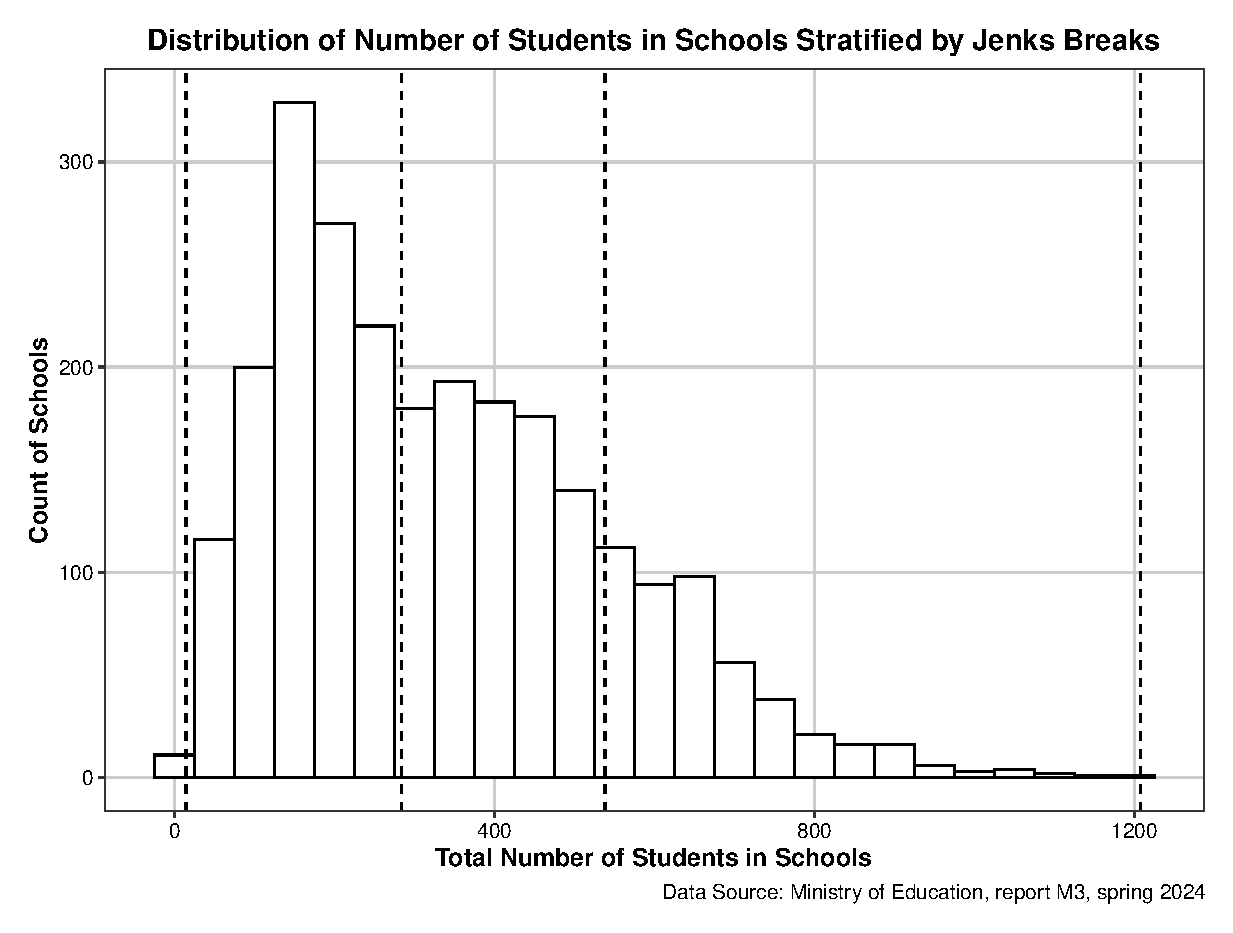
\includegraphics{student_distribution_plot.eps}} \caption{Distribution of student enrolment across schools in the study population, with strata boundaries determined using Jenks Natural Breaks.} \label{school-distribution-plot} \end{figure}


To maintain reproducibility, we employed an R script with a fixed random seed to select the schools included in the sample. Details of the strata distribution, including the number of schools and sample sizes, are presented in Table \ref{strata-distribution}.

\begin{table}
\tbl{Distribution of schools across strata by number of students}
{\begin{tabular}{lccc} \toprule
Stratum & Number of schools & Sample size & Median students \\ \midrule
1 (small schools) & $1,182$ & $158$ & $164.00$ \\
2 (medium schools) & $864$ & $116$ & $400.50$ \\
3 (large schools) & $440$ & $59$ & $641.00$ \\ \midrule
\textbf{Total} & \textbf{$2,486$} & \textbf{$333$} & \\ \bottomrule
\end{tabular}}
\label{strata-distribution}
\end{table}

In the following steps, we aimed to obtain the curricula from all schools in the sample, or at least the section related to the content of History. According to Czech law, school curricula must be publicly accessible; however, the law does not specify the manner in which they should be made accessible. Initially, we attempted to locate the curricula on the schools’ websites. Next, we contacted the schools via email, requesting either their full curriculum or the relevant sections. Finally, we submitted an official request under Czech Act No. 106/1999 Coll. on Free Access to Information. Based on this law, publicly funded schools are required to provide remote access to their curricula. However, this obligation does not apply to private or religious schools.

From July to November 2024, we successfully obtained 321 curricula. Two schools declined our request (the Law on Free Access to Information did not apply due to their status as non-public schools), and ten schools did not respond to our official request. For details regarding the sources from which the school curricula were obtained, see Table \ref{curricula-sources}. With combination of all collection methods, we were able to achieve a very high response rate for the returned curricula.

\begin{table}
\tbl{Sources of school curricula}
{\begin{tabular}{lcc} \toprule
Source & Count & Percentage \\ \midrule
Website & $198$ & $59.46\%$ \\
Mail Request & $43$ & $12.91\%$ \\
Official Request & $80$ & 24.02\% \\ \midrule
\textbf{Returned Curricula} & $321$ & $96.40\%$ \\ \midrule
Refused & $2$ & $0.60\%$ \\ 
No Response & $10$ & $3.00\%$ \\ \midrule
\textbf{Total} & $333$ & $100.00\%$ \\ \midrule
\end{tabular}}
\label{curricula-sources}
\end{table}

Schools provide curricula in various formats (e.g., PDF, HTML, DOCX, DOC, XLSX), often separated by subjects or grades across multiple files. To standardize the input data, we converted all curricula into PDF format, combining multiple files when necessary.


\subsection{Human and LLM Coding Processes}

The goal of this study was twofold: (1) to validate LLM as a viable alternative to human coders for analyzing school curricula, and (2) to identify its limitations and highlight specific contexts in which LLM can be effectively applied. To achieve this, we evaluated LLM performance on three tasks:  
\begin{enumerate}
    \item extracting relevant history content from school curricula PDFs,  
    \item splitting extracted content into discrete topics, and  
    \item labeling topics into broader historical themes aligned with the Czech National Curriculum.  
\end{enumerate}

We compared LLM outputs with those produced by a human coder, who served as the benchmark. The human coder was an experienced lower-secondary history teacher familiar with Czech school curricula structure, terminology, and content.

For LLM processing, we utilized two versions of GPT-4: \texttt{gpt-4o-2024-08-06} and \texttt{gpt-4o-mini-2024-07-18}. These models were selected due to GPT-4's widespread popularity and accessibility. The \texttt{gpt-4o-mini} version offered faster processing and lower costs but operated with a smaller contextual window compared to the full version. This tradeoff is discussed further in the results section.

We evaluated LLM performance based on the following criteria:  
\begin{enumerate}
    \item \textbf{Accuracy}: How closely LLM outputs aligned with human-coded results.  
    \item \textbf{Processing time}: Measured as the total runtime of the LLM processing scripts.  
    \item \textbf{Cost}: Derived directly from OpenLLM’s administrative console based on token usage.  
\end{enumerate}

The following subsections describe each of the three tasks in detail, including the methods applied and the criteria for evaluation.

\subsubsection{Data Extraction}

Due to the absence of a unified format for Czech school curricula, we encountered significant variability in document styles, file sizes, content organization, and terminology. The primary objectives of this task were twofold:  
\begin{enumerate}
    \item To identify the section of the curriculum dedicated to the \textit{History} subject, and  
    \item To extract the relevant content for each grade level.  
\end{enumerate}

Both the LLM models and the human coder were tasked with examining each document, locating the \textit{History} section, and systematically extracting and categorizing all relevant content by grade. These extracted content chunks were later used in subsequent processes, such as topic splitting and labeling.

This step was anticipated to be the most challenging in the data extraction process. Many curricula lacked a table of contents, making it difficult to efficiently locate the relevant \textit{History} section. Furthermore, the organization and presentation of history content varied significantly between schools. Examples of this variability included:  
\begin{itemize}
    \item Curricula presenting the expected learning outcomes and content in a structured table format,  
    \item Curricula combining outcomes and content into a single table cell, and  
    \item Curricula providing content as narrative paragraphs beneath tables listing expected outcomes.  
\end{itemize}

These structural differences posed challenges for both the LLM models and the human coder, as they had to locate, interpret, and extract consistent information across diverse document formats.  

To evaluate the quality of the extracted chunks, we planned to compare the outputs of the LLM models and the human coder using two key metrics:  
\begin{itemize}
    \item \textbf{Total count of extracted chunks}: This metric assesses whether the LLM and human coders extracted a similar number of meaningful units.
    \item \textbf{Character length of extracted chunks}: To evaluate the granularity of extractions, we measured the average and total character lengths of the chunks.
\end{itemize}

To conduct this comparison, a random sample of extracted chunks was selected for detailed analysis. This sampling ensured a fair and representative evaluation of the LLM and human performance in this step of the process.

However, during initial trials of LLM processing the school curricula, we identified significant limitations that rendered LLM unsuitable for this task without extensive customization. These limitations included:  
\begin{itemize}
    \item \textbf{High costs}: Processing the large PDF files using LLM proved financially prohibitive. On average, the school curricula PDFs were $252.23$ pages long (see Figure \ref{figure:pages-distribution-plot} for pages distribution), with an average file size of $2.97$ MB.  
    \item \textbf{Low extraction accuracy}: LLM frequently failed to correctly extract the \textit{History} section of the files. This issue was compounded by the inconsistent organization of the curricula and the lack of a uniform structure across documents.  
\end{itemize}

\begin{figure} \centering \resizebox*{12cm}{!}{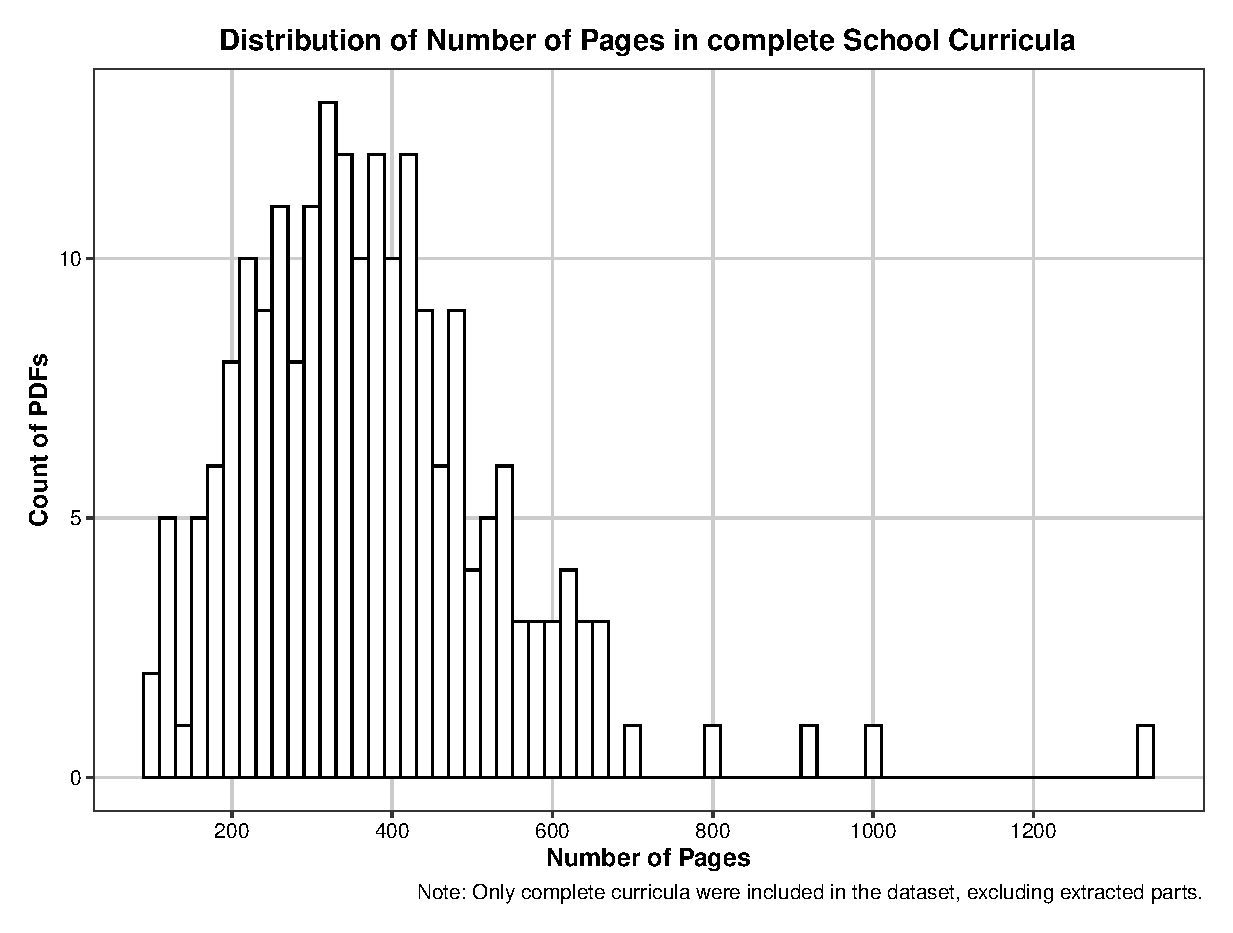
\includegraphics{curricula_pages_distribution_plot.eps}} \caption{Distribution of number of pages of complete school curricula (already extracted History parts have been excluded).} \label{figure:pages-distribution-plot} \end{figure}


Addressing these challenges would require advanced preprocessing, fine-tuning of the LLM models, the use of vector stores, and the development of extensive custom scripts. As a result, we were unable to compare extracted content chunks between LLM and human coders. For the subsequent stages of the project, only the chunks provided by the human coder were used.

\subsubsection{Topic Splitting}

In order to facilitate a meaningful comparison of school curricula, we needed a robust method for identifying and distinguishing individual content topics. Typically, these topics are presented on separate lines in curricula; however, some schools did not clearly separate them, and topics were sometimes embedded within broader sections. Additionally, the definition of what constitutes a single topic varies across curricula, with some topics being more generalized, while others are more specific.

To address this, we split the content into meaningful units. The human coder was used as the baseline for this task, with instructions to follow traditional topic divisions found in Czech history textbooks when determining what constitutes a single topic unit.

For LLM processing, we used a single-shot strategy (TODO: add source on LLM prompting strategy) and provided the following prompt in Czech. The English translation is provided here. See the referenced repository (TODO link to repository) for original prompts:

\begin{quotation}
    The user will provide history curriculum content for a primary school, which may contain inconsistent formatting, transcription errors, and other issues. Reformat the content so that each line corresponds to a distinct and meaningful unit, aligned with the curriculum.
\end{quotation}


We let the LLM process all school curricula, but because this task would be very time-consuming for the human coder, we decided on a smaller sample, even at the cost of a lower confidence level. We used stratified sampling with grades as individual strata and randomly chose 25 content chunks for each grade, resulting in a total sample of 100 content chunks. With 2,186 extracted chunks from previous steps, using a sample size of 100 chunks provides sufficient confidence for this type of analysis, ensuring representativeness and reliability.

We compared the performance of the LLM models against the human coder’s baseline using F1-score, which measures both precision and recall to evaluate how well the models split topics.


\subsubsection{Topic Labeling}

To evaluate the LLM’s ability to label topics, we used predefined labels (referred to as "codes") based on the Czech National Curriculum. Each distinct topic from the school curricula was matched with two labels: one broader history theme label (e.g., '\textit{Earliest Civilizations. Roots of European Culture}') and one more specific topic label (e.g., '\textit{The Oldest Ancient Civilizations...}' or '\textit{Ancient Greece and Rome}'). A complete list of these codes can be found in Appendix \ref{appendix:national-curriculum-topics}. If no predefined label was applicable, the label \textit{other} was used.

Both the human coder and the LLM models had access to this coding table. For the LLM, the table was converted into a markdown list format to facilitate processing. Both the human coder and the LLM models used the content chunks generated by the GPT-4 model in the previous step as input for labeling. 

To ensure accurate labeling, additional context was provided for each content chunk. This included information about the grade level and the original content chunk from the school curriculum. By preserving this contextual information, we aimed to help both the human coder and the LLM models better interpret topics that might otherwise appear ambiguous or dependent on their surrounding content.

To create a manageable dataset for human labeling while ensuring representativeness, we employed a stratified sampling approach. Specifically, we divided the content topics into strata corresponding to the grade levels (grades 6 to 9) and randomly selected 100 topics from each grade, resulting in a total sample of 400 topics. This method ensured that all grade levels were proportionally represented in the evaluation.

The LLM was tasked with labeling the entire set of content topics, while the human coder labeled only the sampled dataset. Importantly, the human coder did not have access to the LLM’s labeling results, ensuring that the evaluation remained unbiased.

To assess the agreement between the human and LLM labels, we computed Cohen’s Kappa, a statistical measure of inter-rater reliability. Cohen’s Kappa accounts for agreement that may occur by chance, providing a robust metric for evaluating labeling consistency. A higher Kappa value indicates stronger agreement. This measure was applied to evaluate both the broader theme and specific topic labels, helping us assess the reliability of the LLM models compared to the human coder.



%% Topic Splitting and Labeling Process: Topic Splitting: Explain how different curricula formats (e.g., lists, paragraphs, tables) were processed to extract topics. Topic Labeling: Describe the broader and specific Czech national curriculum themes, and how "other" categories were applied. %%

%% Human Coding Process. Manual Topic Extraction and Labeling: Detail how human researchers manually split and labeled topics using textbooks and educational expertise. Inter-rater Reliability: Describe how consistency was ensured between multiple coders. Quality Control: Discuss validation checks and human error mitigation. %%

%% LLM Coding Process. Preprocessing: Explain how curricula data was prepared for input into GPT-4o and GPT-4o-mini. Prompt Engineering: Provide examples of prompts used for topic splitting and labeling. LLM Labeling: Detail the process followed by GPT-4o and GPT-4o-mini to split and label topics, and any issues encountered during the process. %%

%% Sampling Strategy. Stratified Sampling: Justify the use of stratified sampling by grades and schools. Random Sample Selection: Describe how the sample for manual coding and evaluation was selected, ensuring representativeness of diverse curricula. %% 

%% Evaluation Metrics. Topic Splitting: Use of F1-score to evaluate topic splitting performance. Topic Labeling: Use of Cohen’s Kappa for evaluating the agreement between human and LLM labeling, and optional use of confusion matrices for deeper insights. %%


\section{Results}



%% Briefly introduce the main goals of the results section: comparing the performance of human coders and LLM (GPT-4o and GPT-4o-mini) in terms of topic splitting and labeling. %% 

\subsection{Data Extracting}




\subsection{Topic Splitting: Performance Comparison}

to Table \ref{table:llm-costs} note that mention that time is approximate depending on network conditions, speed and utilization of OpenAI servers.

\begin{table}
\tbl{Processing Times and Costs of LLM Models}{
\begin{tabular}{lcc} \toprule
\textbf{LLM Model} & \textbf{Processing Time} & \textbf{Cost (USD)} \\ \midrule
\texttt{gpt-4o-2024-08-06} & Approximately $9$ hours & $31.24$ \\
\texttt{gpt-4o-mini-2024-07-18} & Approximately $6$ hours & $1.56$ \\ \bottomrule
\end{tabular}}
\label{table:llm-costs}
\end{table}



%% F1-Score Results: Present the F1-scores for both human coders and LLM (GPT-4o and GPT-4o-mini) for the task of splitting topics. Use tables or graphs to visually compare the F1-scores for different LLM models and human coding (e.g., bar graphs or scatter plots). Discuss how these scores reflect the accuracy of LLM in detecting and splitting topics compared to human coders. %%

%% Precision and Recall Breakdown (Optional). If relevant, break down the precision and recall scores for LLM vs. human coders and discuss their significance. %%

%% Error Analysis: Analyze where LLM and human coders made errors (e.g., false positives, false negatives). Provide examples of common mistakes made by LLM or human coders, using specific curricula or topics as illustrations. Discuss possible reasons for discrepancies and potential areas of improvement. %%

\subsection{Topic Labeling: Performance Comparison}

See table \ref{table:national-curriculum-topics} in appendix \ref{appendix:national-curriculum-topics} with topics of national curriculum for History.


%% Cohen’s Kappa Results: Present the Cohen’s Kappa values for both human-LLM agreement and human-human agreement (if applicable), comparing them across different LLM models. Provide visual representations (e.g., box plots, heat maps) to highlight any significant differences in agreement levels. Discuss what the Cohen's Kappa values suggest about the consistency of the labeling process for human coders vs. LLM models. %%


\section{Discussion}


%% Interpretation of Key Findings: Summarize the most important results, highlighting any notable differences or trends between human coding and LLM coding performance. Discuss the implications of these results for future curriculum analysis, particularly in terms of the role of LLM in educational research. %%

%% Limitations of the Results: Acknowledge any limitations in the results, such as sample size, potential biases in the dataset, or constraints in the LLM models used. %%

- provide in prompt to topic splitting list of possible topics, use vector store

%% Suggestions for Future Research: Suggest areas where LLM models could be improved to handle the challenges identified in the study. Propose potential future studies to further assess LLM’s applicability in analyzing educational data and curriculum content. %%


\section{Conclusion}

%% Summary of Findings: Recap the major conclusions drawn from the results, emphasizing the overall performance of LLM in comparison to human coding. %%

%% Implications for Curriculum Analysis: Briefly mention the broader impact of these findings on automating curriculum analysis and improving the efficiency of educational research. %%


\bibliographystyle{apacite}
\bibliography{bibliography}


\section{Appendices}

\appendix

\section{History Topics from the Czech National Curriculum}
\label{appendix:national-curriculum-topics}

\setcounter{table}{0}
\begin{sidewaystable}
 \tbl{History Topics Defined in the Czech National Curriculum}
  {\begin{tabular}{r|p{10cm}|p{10cm}}

\textbf{Code} & \textbf{Topic (Czech)} & \textbf{Topic (English)} \\ \hline \hline
\textbf{A} & \textbf{ČLOVĚK V DĚJINÁCH} & \textbf{HUMANITY IN HISTORY} \\
A1 & význam zkoumání dějin, získávání informací o dějinách; historické prameny & the importance of studying history, obtaining historical information; historical sources \\ 
A2 & historický čas a prostor & historical time and space \\ \hline

\textbf{B} & \textbf{POČÁTKY LIDSKÉ SPOLEČNOSTI} & \textbf{THE ORIGINS OF HUMAN SOCIETY} \\ 
B1 & člověk a lidská společnost v pravěku & humans and society in prehistory \\ \hline

\textbf{C} & \textbf{NEJSTARŠÍ CIVILIZACE. KOŘENY EVROPSKÉ KULTURY} & \textbf{EARLIEST CIVILIZATIONS. ROOTS OF EUROPEAN CULTURE} \\ 
C1 & nejstarší starověké civilizace a jejich kulturní odkaz & the oldest ancient civilizations and their cultural legacy \\ 
C2 & antické Řecko a Řím & ancient Greece and Rome \\ 
C3 & střední Evropa a její styky s antickým Středomořím & Central Europe and its ties to the ancient Mediterranean \\ \hline

\textbf{D} & \textbf{KŘESŤANSTVÍ A STŘEDOVĚKÁ EVROPA} & \textbf{CHRISTIANITY AND MEDIEVAL EUROPE} \\
D1 & nový etnický obraz Evropy & the new ethnic composition of Europe \\ \hline
D2 & utváření států ve východoevropském a západoevropském kulturním okruhu a jejich specifický vývoj & the formation of states in Eastern and Western Europe and their specific developments \\ 
D3 & islám a islámské říše ovlivňující Evropu (Arabové, Turci) & Islam and Islamic empires influencing Europe (Arabs, Turks) \\ 
D4 & Velká Morava a český stát, jejich vnitřní vývoj a postavení v Evropě & Great Moravia and the Czech state, their internal development and position in Europe \\ 
D5 & křesťanství, papežství, císařství, křížové výpravy & Christianity, the Papacy, the Empire, the Crusades \\ 
D6 & struktura středověké společnosti, funkce jednotlivých vrstev & structure of medieval society, functions of individual social classes \\ 
D7 & kultura středověké společnosti - románské a gotické umění a vzdělanost & culture of medieval society - Romanesque and Gothic art and education \\ \hline

\textbf{E} & \textbf{OBJEVY A DOBÝVÁNÍ. POČÁTKY NOVÉ DOBY} & \textbf{DISCOVERIES AND CONQUESTS. BEGINNINGS OF THE MODERN ERA} \\ 
E1 & renesance, humanismus, husitství, reformace a jejich šíření Evropou & Renaissance, humanism, Hussite movement, Reformation, and their spread across Europe \\ 
E2 & zámořské objevy a počátky dobývání světa & overseas discoveries and the beginnings of global conquest \\ 
E3 & český stát a velmoci v 15.-18. století & the Czech state and great powers in the 15th-18th centuries \\ 
E4 & barokní kultura a osvícenství & Baroque culture and the Enlightenment \\ \hline

\textbf{F} & \textbf{MODERNIZACE SPOLEČNOSTI} & \textbf{MODERNIZATION OF SOCIETY} \\ 
F1 & Velká francouzská revoluce a napoleonské období, jejich vliv na Evropu a svět; vznik USA & the French Revolution and the Napoleonic era, their impact on Europe and the world; the founding of the USA \\ 
F2 & industrializace a její důsledky pro společnost; sociální otázka & industrialization and its consequences for society; the social question \\ 
F3 & národní hnutí velkých a malých národů; utváření novodobého českého národa & national movements of large and small nations; the formation of the modern Czech nation \\ 
F4 & revoluce 19. století jako prostředek řešení politických, sociálních a národnostních problémů & revolutions of the 19th century as a means of solving political, social, and national issues \\ \hline

\textbf{G} & \textbf{MODERNÍ DOBA} & \textbf{THE MODERN ERA} \\ 
G1 & první světová válka a její politické, sociální a kulturní důsledky & the First World War and its political, social, and cultural consequences \\ 
G2 & nové politické uspořádání Evropy a úloha USA ve světě; vznik Československa, jeho hospodářsko-politický vývoj, sociální a národnostní problémy & the new political order in Europe and the role of the USA; the formation of Czechoslovakia, its economic-political development, and social and national issues \\ \hline

\textbf{H} & \textbf{ROZDĚLENÝ A INTEGRUJÍCÍ SE SVĚT} & \textbf{A DIVIDED AND INTEGRATING WORLD} \\ 
H1 & studená válka, rozdělení světa do vojenských bloků reprezentovaných supervelmocemi; politické, hospodářské, sociální a ideologické soupeření & the Cold War, division of the world into military blocs represented by superpowers; political, economic, social, and ideological competition \\ 
H2 & vývoj Československa od roku 1945 do roku 1989, vznik České republiky & the development of Czechoslovakia from 1945 to 1989, the establishment of the Czech Republic \\
\end{tabular}}\tabnote{Source: \cite{RVPZV2023}}\label{table:national-curriculum-topics}

\end{sidewaystable}



\end{document}
